%===============================================================================
% Technical Environnement
%===============================================================================
\newpage{}
\chapter{Environnement de développement}

%+++++++++++++++++++++++++++++++++++++++++++++++++++++++++++++++++++++++++++++++
\section{Eclipse - indigo}
%+++++++++++++++++++++++++++++++++++++++++++++++++++++++++++++++++++++++++++++++
Le développement de \youTestIt{} est réalisé sous eclipse avec différents plugins afin de standardiser 
le code. Il est préférable pour toutes contributions d'utiliser un environnement similaires.

La version utiliser doit être une version supérieur ou égale à \textbf{indigo}. 

Liste des plugins :
\begin{itemize}
	\item JBoss tools : qui permet l'intégration simple de jboss 7 ainsi que des outils pour Seam.
				Le plugin est présent sur le marcket place d'eclipse.
				
	\item Maven Integration for Eclipse : pour la gestion des dépendances.
					Le plugin est présent sur le marcket place d'eclipse.
					
	\item EGit : pour la gestion des sources sous GitHub
					Le plugin est présent sur le marcket place d'eclipse.
					
	\item PMD : pour la vérification du code
					Le plugin s'installe via l'adresse \textbf{http://pmd.sourceforge.net/eclipse } à rajouter dans 
					le menu software update d'eclipse.
					
	\item Check style : pour la vérification du code
					Le plugin est présent sur le marcket place d'eclipse.
					
	\item Grep Console : non obligatoire, mais facilite la lecture de la console
					Le plugin est présent sur le marcket place d'eclipse.
\end{itemize}

\paragraph{Formatage du code :}
Il est très important de configurer eclipse avec les différents fichiers de formatages
présent dans le projet. 

On retrouve cinq fichiers de configuration :
\begin{itemize}
	\item  \textbf{cleanups.xml :}  Se configure dans :
				  preferences $\rightarrow$ Java $\rightarrow$Code Style$\rightarrow$Clean up

	\item \textbf{codetemplates.xml :}  Se configure dans :
				 preferences $\rightarrow$ Java $\rightarrow$Code Style$\rightarrow$Code template

	\item \textbf{formatter.xml :} Se configure dans :
				 preferences $\rightarrow$ Java $\rightarrow$Code Style$\rightarrow$Formatter

	\item  \textbf{pmd.xml :} Pour tous les projets importés il faut aller dans leurs propriétés  
		(clique droit sur le projet$\rightarrow$Properties ).
		\begin{enumerate}
			\item aller dans le menu PMD
			\item cliquer sur "activer PMD"
			\item il faut en suite cliquer sur \emph{Utiliser l'ensemble des règles configuré dans un fichier projet}
			\item cliquer sur parcourir pour rechercher le fichier de configuration du projet.
			\item valider le formulaire.
		\end{enumerate}


	\item  \textbf{checkstyle.xml :}
		Pour le configurer il faut suivre les étapes suivantes :
		\begin{enumerate}
				\item aller dans les préférences d'eclipse
				\item aller dans menu Checkstyle
				\item cliquer sur new
				\item une nouvelle fenêtre s'ouvre, il faut choisir \textbf{External Configuration File}
				\item donner un nom à la configuration
				\item cliquer sur \textbf{Browse...} pour aller rechercher le fichier checkstyle.xml du projet \youTestIt{}.
				\item valider le formulaire.
				\item définisser la nouvelle configuration comme configuration par défaut (\textbf{Set as Default})
				\item A présent pour chaque projet importer il faut aller sans sa configuration 
							(clique droit sur le projet$\rightarrow$Properties )
				\item Dans le menu Checkstyle  il faut choisir la configuration  \youTestIt{} et valider le formulaire.
		\end{enumerate}
	

	\paragraph{}	
	
	\begin{attention}
		Toute contribution ne respectant pas les conventions de formatage ne sera pas prit en compte.
	\end{attention}
	
\end{itemize}
%+++++++++++++++++++++++++++++++++++++++++++++++++++++++++++++++++++++++++++++++
\section{GitHub}
%+++++++++++++++++++++++++++++++++++++++++++++++++++++++++++++++++++++++++++++++
L'ensemble du code source du projet se trouve sur GitHub. Pour pouvoir contribuer il est
nécessaire d’être inscrit sur le site.  Une fois inscrit il faut crée et uploader sa clé RSA, pour cela il faut suivre le tutoriel proposé 
par GitHub : \href{http://help.github.com/linux-set-up-git/ }{http://help.github.com/linux-set-up-git}. 

une fois le compte gitHub configuré, il suffit de faire une demande d'ajout par mail à l'adresse
\textbf{administrator@youtestit.org}, pour que l'on vous rajoute au projet.

\subsection{Configuration eclipse pour GitHub}
Une fois ajouter sur le projet  vous pouvez récupérer les sources et commencer à contribuer. 
Mais avant cela il faut encore configurer eclispe pour avoir un environnement de développement
fonctionnel. 

\begin{enumerate}
	\item créer un dossier dans votre home (par exemple : /home/yourLogin/git ). Ce dossier contiendra
	 l'ensemble des sources du projet.
	 
	\item Il faut ensuite cloner tous les projets dans ce dossier
	 \lstsetSh{}
	 \lstinputlisting{includes/src/gitClone.sh}
	 
	 \item Le plugin EGit fonctionne très mal avec la librairie SSH d'eclipse, il faut impérativement lui
	 ordonner de travailler avec la librairie système. Pour cela il faut  crée un script shell pour le lancement
	 d'éclispe qui va initialiser les bonnes variables d'environnement.
	 
	 \lstsetSh{}
	 \lstinputlisting{includes/src/eclipse.sh}
	On en profite également pour spécifier l'emplacement de maven et du JDK.
	\newpage

	 \item Une fois eclipse démarrer on va pouvoir récupérer nos dépôt git. Dans la perspective
	 Git repository exploring, on peut rajouter un dépôt en cliquant sur l'icone avec un + vert.
		\begin{figure}[!h]
     		\begin{center}
			      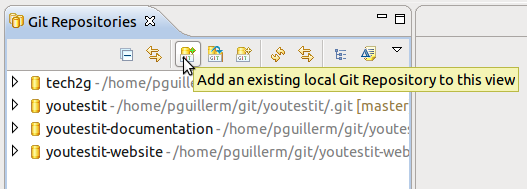
\includegraphics[width=0.5\textwidth]{gitAdd}
			      \caption{Ajout d'un dépôt Git}
			      \label{gitAdd}
		    \end{center}
		\end{figure}
		
	 \item Une nouvelle fenêtre s'ouvre dans la quel on va pouvoir aller chercher  l'emplacement du
	 dépôt Git locale. Le bouton "seach" permet au plugin d'aller récupérer le .git du dépôt. Il ne 
	 reste plus qu'à valider le formulaire.
		\begin{figure}[!h]
     		\begin{center}
			      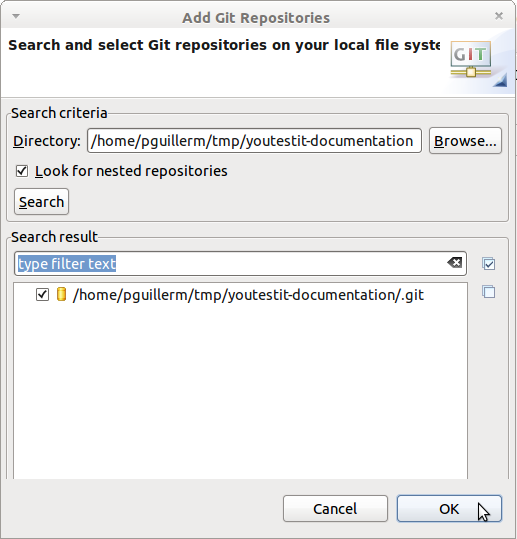
\includegraphics[width=0.5\textwidth]{gitRepo}
			      \caption{Récupération des dépôt Git}
			      \label{gitAddRepo}
		    \end{center}
		\end{figure}	
		\newpage
	 
	 \item Git a besoin d'une connexion SSH avec une clé RSA pour fonctionner. Il faut
	 bien vérifier que la configuration eclipse pour SSH est correcte et qu'elle contient
	 bien la clé RSA.
		\begin{figure}[!h]
     		\begin{center}
			      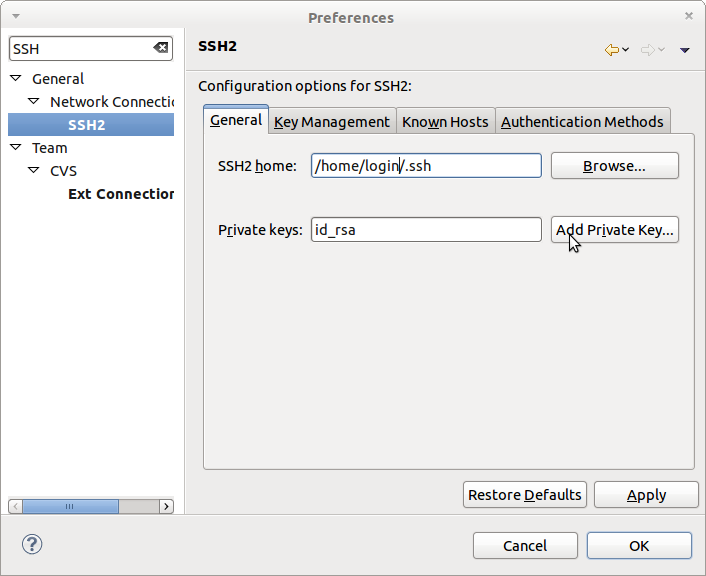
\includegraphics[width=0.5\textwidth]{sshParams}
			      \caption{Configuration SSH d'eclipse}
			      \label{eclipseSshConfig}
		    \end{center}
		\end{figure}		 
	 
	\item Une fois la configuration terminée, vous pouvez importer les projets en tant que "general project" .
	Pour cela il suffit de déplier le dépôt et de faire un clique droit sur le "Working directory" .
		\begin{figure}[!h]
     		\begin{center}
			      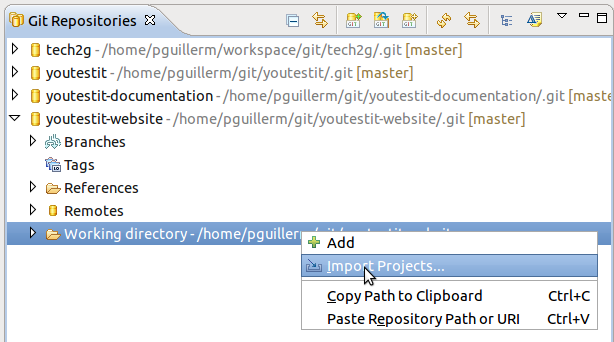
\includegraphics[width=0.5\textwidth]{importProject}
			      \caption{Importation d'un projet}
			      \label{gitProjectImport}
		    \end{center}
		\end{figure}	
		
	\item Votre environnement est prêt à faire de pull et push ;)   Pour plus  d'information je vous invite à lire la
	documentation du plugin Egit : \href{http://wiki.eclipse.org/EGit/User\_Guide}{http://wiki.eclipse.org/EGit/User\_Guide} . 
 
	 
\end{enumerate}

%+++++++++++++++++++++++++++++++++++++++++++++++++++++++++++++++++++++++++++++++
\section{youtestit-documentation}
%+++++++++++++++++++++++++++++++++++++++++++++++++++++++++++++++++++++++++++++++


%+++++++++++++++++++++++++++++++++++++++++++++++++++++++++++++++++++++++++++++++
\section{youtestit-website}	
%+++++++++++++++++++++++++++++++++++++++++++++++++++++++++++++++++++++++++++++++


%+++++++++++++++++++++++++++++++++++++++++++++++++++++++++++++++++++++++++++++++
\section{youtestit}
%+++++++++++++++++++++++++++++++++++++++++++++++++++++++++++++++++++++++++++++++

